\documentclass[11pt,a4paper]{article}
\usepackage[margin=21mm,headheight=16pt,footskip=12mm]{geometry}
\usepackage[T1]{fontenc}
\usepackage{lmodern}
\renewcommand{\familydefault}{\sfdefault}
\usepackage{microtype,graphicx,xcolor,booktabs,tabularx,array,enumitem,fancyhdr}
\usepackage[most]{tcolorbox}
\usepackage{tikz}
\usetikzlibrary{arrows.meta,positioning,calc,matrix}
\usepackage{hyperref}
\definecolor{forest}{HTML}{155C34}
\definecolor{neon}{HTML}{69F05B}
\definecolor{mint}{HTML}{EDF7EF}
\definecolor{ink}{HTML}{18261E}
\definecolor{muted}{HTML}{53655A}
\definecolor{line}{HTML}{CADCCE}
\definecolor{gold}{HTML}{B68B24}
\definecolor{palegold}{HTML}{FBF6E8}
\color{ink}
\hypersetup{colorlinks=true,linkcolor=forest,urlcolor=forest,pdftitle={MiniDavis: Presentation Guide},pdfauthor={MiniDavis Team},pdfsubject={Plain-language explanations, speaker notes and demo instructions}}
\graphicspath{{../assets/}}
\newcolumntype{Y}{>{\raggedright\arraybackslash}X}
\newcolumntype{P}[1]{>{\raggedright\arraybackslash}p{#1}}
\setlength{\parindent}{0pt}
\setlength{\parskip}{6pt}
\setlist[itemize]{leftmargin=*,itemsep=4pt,topsep=4pt}
\setlist[enumerate]{leftmargin=*,itemsep=5pt,topsep=4pt}
\pagestyle{fancy}
\fancyhf{}
\fancyhead[L]{\small\ttfamily\color{forest} MINIDAVIS / PRESENTATION GUIDE}
\fancyhead[R]{\small\color{muted} A tiny town for AI agents}
\fancyfoot[L]{\footnotesize\color{muted} Explain the idea. Show the evidence. Keep the demo simple.}
\fancyfoot[R]{\small\thepage}
\renewcommand{\headrulewidth}{0.3pt}
\newcommand{\pagehead}[3]{\clearpage{\color{forest}\small\ttfamily #1 \hfill #3}\par\vspace{3pt}{\LARGE\bfseries #2}\par\vspace{5pt}}
\newcommand{\subhead}[1]{\par\vspace{7pt}\noindent{\large\bfseries\color{forest}#1}\par\nobreak\vspace{2pt}}
\newcommand{\keyline}[1]{\begin{tcolorbox}[colback=ink,colframe=ink,arc=2mm,boxrule=0pt,left=4mm,right=4mm,top=3mm,bottom=3mm]\color{white}\bfseries #1\end{tcolorbox}}
\newtcolorbox{saybox}{colback=mint,colframe=forest,boxrule=.5pt,arc=2mm,left=3mm,right=3mm,top=2mm,bottom=2mm,fonttitle=\bfseries,title=Suggested words}
\newtcolorbox{notebox}[1]{colback=palegold,colframe=gold,boxrule=.4pt,arc=2mm,left=3mm,right=3mm,top=2mm,bottom=2mm,fonttitle=\bfseries,title=#1}
\newcommand{\captiontext}[1]{{\footnotesize\color{muted}#1\par}}
\newcommand{\handoff}[1]{\vfill{\small\color{forest}\textbf{Hand-off:} #1}\par}
\newcommand{\screen}[2]{\begin{center}\includegraphics[width=\linewidth,height=#2,keepaspectratio]{#1}\end{center}}
\tikzset{card/.style={draw=line,fill=mint,rounded corners=3pt,align=center,inner sep=7pt,minimum height=1.1cm,text width=3.5cm,font=\small},darkcard/.style={card,fill=ink,text=white,draw=ink},arr/.style={-{Stealth[length=2.5mm]},thick,draw=forest}}
\begin{document}

\thispagestyle{empty}
\begin{tcolorbox}[colback=ink,colframe=ink,arc=0mm,boxrule=0pt,left=6mm,right=6mm,top=7mm,bottom=7mm]
{\color{neon}\ttfamily\fontsize{34}{39}\selectfont\bfseries MiniDavis}\par\vspace{4mm}
{\color{white}\LARGE A tiny town for AI agents.}\par\vspace{3mm}
{\color{neon}\large Presentation guide}\par
\end{tcolorbox}
\screen{demo-recorded.jpg}{10cm}
\captiontext{The simplified interface, showing a clearly labelled recorded example. Live AI decisions and the recorded example are separate parts of the demonstration.}
\vspace{4mm}
{\Large\bfseries Tell the story before naming the technology.}\par
This guide helps the team explain MiniDavis to people who have never studied machine learning. It contains slide ideas, plain-language explanations, suggested speaking notes, diagrams, demo steps and answers to likely questions.
\begin{tcolorbox}[colback=mint,colframe=line,boxrule=.4pt,arc=2mm]
\textbf{Audience promise:} Someone should leave able to explain what an agent does, how a stored memory helps it choose, and why classifying an interaction is different from deciding an action.
\end{tcolorbox}
\vfill
{\small\color{muted}Team: Eric, Saurya, Rylee, Ethan, Gayatri and Aishani.\\The speaker assignments follow the team's requested division of topics.}

\pagehead{GUIDE MAP}{Who explains what}{Team reference}
\label{roles}
\begin{tabularx}{\linewidth}{@{}P{3.7cm}P{3cm}Y@{}}
\toprule
\textbf{Section} & \textbf{Presenter} & \textbf{Audience takeaway}\\
\midrule
Frontend & Saurya & The town and stories are our window into the simulation.\\
Backend & Rylee & World rules decide what can actually happen.\\
RAG and memories & Ethan & Agents can look up relevant past events before deciding.\\
Classifier & Gayatri & A smaller trained model sorts interactions into four categories.\\
Live demo & Aishani / Saurya & Watch a real action, then a labelled recorded exchange.\\
Further development & Aishani & Explain what to improve and how to measure progress.\\
\bottomrule
\end{tabularx}
Eric can introduce the project, connect the sections and close the presentation as team lead.

\subhead{How to use this guide}
\begin{enumerate}
\item \textbf{Use diagrams as slide blueprints.} Keep the main idea and a few labels on the actual slide.
\item \textbf{Adapt the suggested words.} These are speaking notes, not paragraphs to paste onto slides.
\item \textbf{Learn your hand-off.} End by setting up the next person's question.
\item \textbf{Prepare off-stage.} Model setup, memory inspectors, API details and diagnostics stay under \textbf{Presenter tools}.
\item \textbf{Keep evidence and examples distinct.} A diagram is an explanation; a screenshot shows an app state; a recorded example does not prove autonomous cooperation.
\end{enumerate}
\keyline{One recurring story: a resident has a goal, checks the world, recalls relevant facts, proposes an action, and acts only if the world allows it.}
\subhead{Language that helps}
Say "a virtual resident" before "an agent." Say "look up a useful memory" before "retrieval-augmented generation." Say "sort a sentence into a category" before "classification." Introduce the technical term after the everyday explanation.
\subhead{Language to avoid}
Do not say residents are conscious, that every animation frame calls an AI model, that memory automatically retrains the model, or that a predicted label changes the town's rules.

\pagehead{OPENING}{Start with the town, not the stack}{Eric / host}
\label{opening}
\keyline{MiniDavis is a small, visible world where we can observe decisions and their consequences.}
\begin{center}
\resizebox{\linewidth}{!}{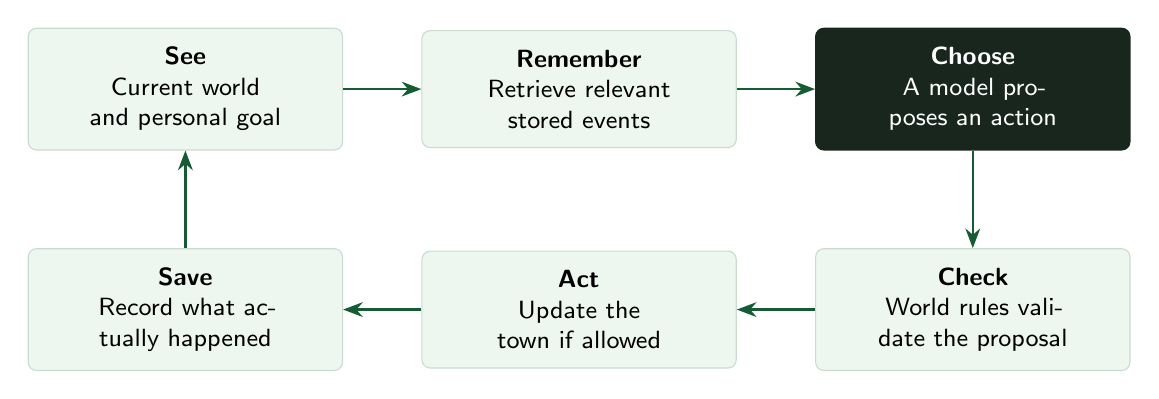
\begin{tikzpicture}
\node[card] (see) at (0,0) {\textbf{See}\\Current world and personal goal};
\node[card] (remember) at (5,0) {\textbf{Remember}\\Retrieve relevant stored events};
\node[darkcard] (choose) at (10,0) {\textbf{Choose}\\A model proposes an action};
\node[card] (save) at (0,-2.8) {\textbf{Save}\\Record what actually happened};
\node[card] (act) at (5,-2.8) {\textbf{Act}\\Update the town if allowed};
\node[card] (check) at (10,-2.8) {\textbf{Check}\\World rules validate the proposal};
\draw[arr] (see)--(remember);\draw[arr] (remember)--(choose);\draw[arr] (choose)--(check);
\draw[arr] (check)--(act);\draw[arr] (act)--(save);\draw[arr] (save)--(see);
\end{tikzpicture}}
\end{center}
\captiontext{Conceptual agent loop. Animation is a visual layer over discrete, validated world turns.}
\begin{saybox}
Imagine a tiny town with five residents. They can collect supplies, move around, speak and exchange resources. Each has a goal, but the interesting part is watching how a decision becomes an action in the world.

An agent is a software character that observes a situation and chooses what to do next. It is not a person inside the computer. In MiniDavis, a language model can suggest an action, memories can supply context, and the town checks whether the action is legal.

We wanted something people could watch instead of another chat box. You can select a resident, follow its story, and see what actually happened. We will explain the system behind that picture, then demonstrate it.
\end{saybox}
\subhead{Opening slide idea}
The title, a town screenshot and the question: \textbf{"How do goals, memories and rules shape an AI agent's choices?"}
\handoff{"Saurya will show how we made those choices visible."}

\pagehead{FRONTEND}{A window into the town}{Saurya}
\label{frontend}
\screen{demo-recorded.jpg}{8.5cm}
\captiontext{Actual audience view of a recorded, scripted example. Source IDs, model diagnostics, setup fields and classifier testing are hidden.}
\begin{tabularx}{\linewidth}{@{}>{\bfseries}P{3.3cm}Y@{}}
The town & Locations and resident positions make each turn visible.\\
Resident stories & Select a name to see its goal, supplies and executed actions.\\
Simple controls & Play/Pause, Next Turn, Reset and a labelled Recorded example.\\
\end{tabularx}
\begin{saybox}
The frontend is the part people see and click. Think of it as a window into the town. The left side shows the world, and the right side follows the resident we select.

We used React to organize the screen into reusable pieces, such as the map, residents and story panel. React is a tool for building interactive interfaces. It does not make the residents intelligent.

The important design choice is that the screen displays the backend's real state. When a turn completes, the new positions and actions appear. Animation makes those updates easier to follow, but the picture does not decide what happens.

For the demo, we keep the controls simple. The deeper memory, classifier and setup tools remain available to presenters without competing for the audience's attention.
\end{saybox}
\handoff{"Rylee will explain who decides whether an action is allowed."}

\pagehead{BACKEND}{The world is the referee}{Rylee}
\label{backend}
\begin{center}
\resizebox{\linewidth}{!}{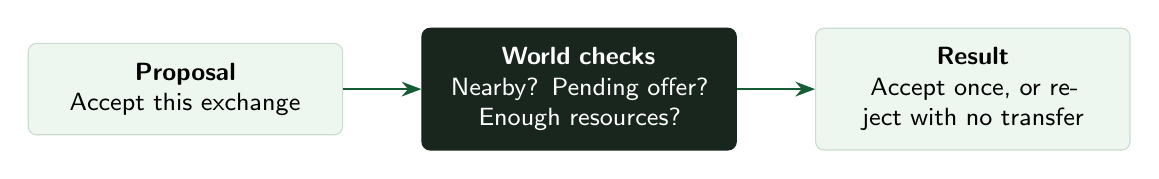
\begin{tikzpicture}
\node[card] (p) at (0,0) {\textbf{Proposal}\\Accept this exchange};
\node[darkcard] (r) at (5,0) {\textbf{World checks}\\Nearby? Pending offer? Enough resources?};
\node[card] (e) at (10,0) {\textbf{Result}\\Accept once, or reject with no transfer};
\draw[arr] (p)--(r);\draw[arr] (r)--(e);
\end{tikzpicture}}
\end{center}
\subhead{A concrete exchange}
\begin{tabularx}{\linewidth}{@{}lYY@{}}
\toprule & \textbf{Before} & \textbf{After}\\\midrule
Ethan & 3 food, 10 coins & 2 food, 11 coins\\
Saurya & 3 food, 6 coins & 4 food, 5 coins\\
Total & 6 food, 16 coins & 6 food, 16 coins\\
\bottomrule
\end{tabularx}
\captiontext{Inventory arithmetic from the scripted fixture. A sentence cannot create food or money; the engine conserves transferred resources.}
\begin{saybox}
The backend is the part working behind the screen. Our Python world engine is the referee. The AI can suggest something, but it cannot directly change its food, coins or position.

For a trade, the engine checks that an offer exists, that the correct resident accepts, that the residents are nearby, and that both sides can pay. A valid exchange happens once. Repeating the acceptance cannot transfer resources again.

Movement and gathering follow the same principle: check the rules before changing anything, then write a factual event.

FastAPI is the messenger between the interface and that engine. A button requests a turn, and the service returns the updated state. We can test these rules even when the AI service is unavailable. We also reuse travel plans rather than calling a model for every animation step.
\end{saybox}
\begin{notebox}{Keep this distinction clear}
An AI explanation is commentary about a proposal. A recorded event is what the engine executed. Relationship changes follow fixed exchange rules, independently of classifier predictions.
\end{notebox}
\handoff{"Here is how that referee connects to the AI and memory."}

\pagehead{SYSTEM VIEW}{Different tools do different jobs}{Rylee}
\label{architecture}
\begin{center}
\resizebox{\linewidth}{!}{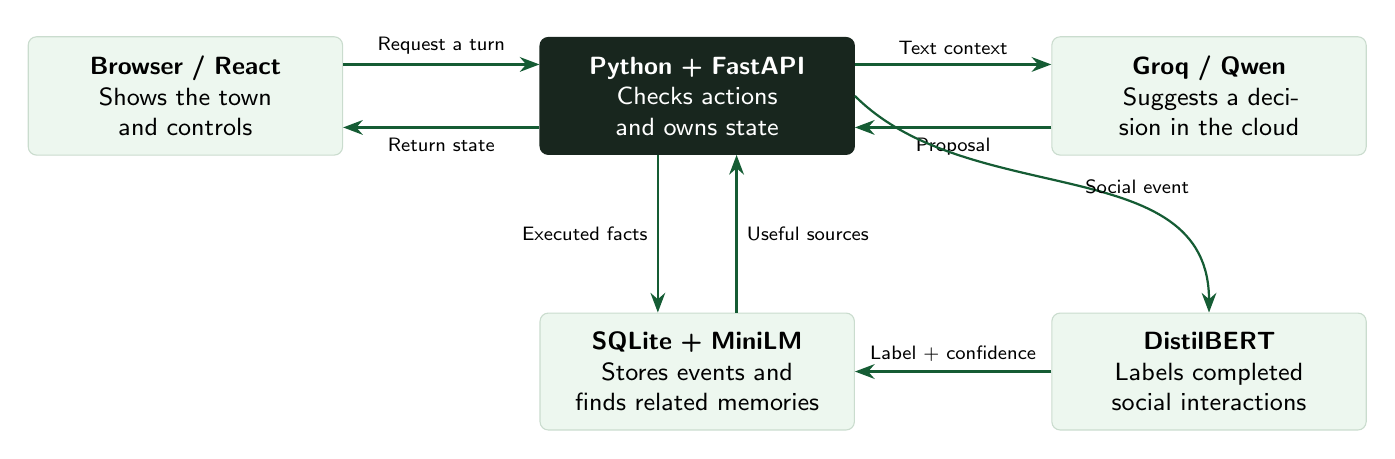
\begin{tikzpicture}
\node[card] (ui) at (0,0) {\textbf{Browser / React}\\Shows the town and controls};
\node[darkcard] (world) at (6.5,0) {\textbf{Python + FastAPI}\\Checks actions and owns state};
\node[card] (cloud) at (13,0) {\textbf{Groq / Qwen}\\Suggests a decision in the cloud};
\node[card] (memory) at (6.5,-3.5) {\textbf{SQLite + MiniLM}\\Stores events and finds related memories};
\node[card] (classifier) at (13,-3.5) {\textbf{DistilBERT}\\Labels completed social interactions};
\draw[arr] ([yshift=4mm]ui.east)--node[above,font=\scriptsize]{Request a turn} ([yshift=4mm]world.west);
\draw[arr] ([yshift=-4mm]world.west)--node[below,font=\scriptsize]{Return state} ([yshift=-4mm]ui.east);
\draw[arr] ([yshift=4mm]world.east)--node[above,font=\scriptsize]{Text context} ([yshift=4mm]cloud.west);
\draw[arr] ([yshift=-4mm]cloud.west)--node[below,font=\scriptsize]{Proposal} ([yshift=-4mm]world.east);
\draw[arr] ([xshift=-5mm]world.south)--node[left,font=\scriptsize]{Executed facts} ([xshift=-5mm]memory.north);
\draw[arr] ([xshift=5mm]memory.north)--node[right,font=\scriptsize]{Useful sources} ([xshift=5mm]world.south);
\draw[arr] (world.east) to[out=-45,in=90] node[right,font=\scriptsize]{Social event} (classifier.north);
\draw[arr] (classifier.west)--node[above,font=\scriptsize]{Label + confidence} (memory.east);
\end{tikzpicture}}
\end{center}
\subhead{The three AI-related jobs}
\begin{tabularx}{\linewidth}{@{}P{2.7cm}P{4.3cm}Y@{}}
\toprule\textbf{Job} & \textbf{Tool} & \textbf{Everyday description}\\\midrule
Choose & Hosted Qwen through Groq & A planner proposing an action.\\
Find memory & MiniLM and our retrieval code & A librarian finding related stored events.\\
Categorize & Fine-tuned DistilBERT & A sorter attaching an interaction label.\\
\bottomrule
\end{tabularx}
\begin{saybox}
These tools are not doing the same job. The language model suggests a decision. The memory system finds past facts. The classifier labels an interaction after it happens.

The five residents share one hosted language-model service but receive separate observations and memory contexts. We do not run five large models on a laptop. The backend can run the smaller memory and classification models on a CPU.

Groq is the service; Qwen is the decision model it hosts. That model receives text and numbers about the world. It is not looking at the pixel-art screenshot. The screenshot is for us.
\end{saybox}
\handoff{"Ethan will explain how a stored event becomes a useful memory."}

\pagehead{MEMORIES}{A notebook of things that actually happened}{Ethan}
\label{memories}
\begin{center}
\resizebox{\linewidth}{!}{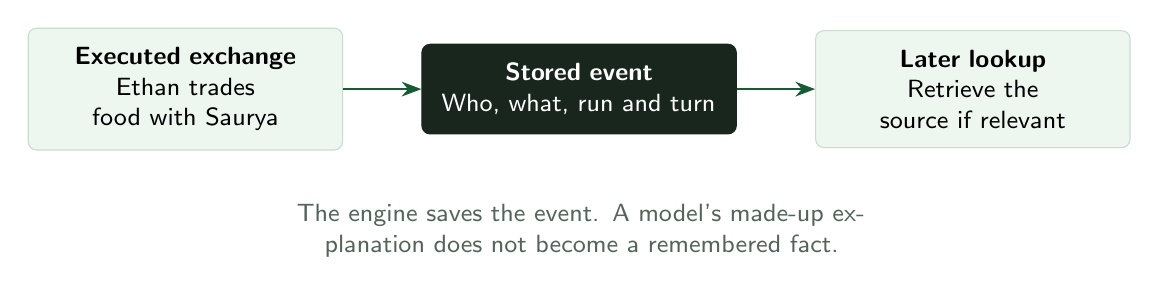
\begin{tikzpicture}
\node[card] (a) at (0,0) {\textbf{Executed exchange}\\Ethan trades food with Saurya};
\node[darkcard] (b) at (5,0) {\textbf{Stored event}\\Who, what, run and turn};
\node[card] (c) at (10,0) {\textbf{Later lookup}\\Retrieve the source if relevant};
\draw[arr] (a)--(b);\draw[arr] (b)--(c);
\node[align=center,font=\small,text=muted,text width=12cm] at (5,-1.8) {The engine saves the event. A model's made-up explanation does not become a remembered fact.};
\end{tikzpicture}}
\end{center}
\subhead{What a memory needs}
\begin{itemize}
\item \textbf{A fact:} the executed action and result.
\item \textbf{An owner:} the resident who experienced it. Both participants can have their own source copy.
\item \textbf{A boundary:} the right run and an event that has already happened.
\item \textbf{A source ID:} a way to inspect the original record in presenter tools.
\end{itemize}
\begin{saybox}
A memory is not a mysterious second brain. It is a saved record of an event. If Ethan and Saurya complete a trade, the engine records who exchanged what and when it happened.

We store records in SQLite, which is a small, organized filing cabinet. Before a later decision, our code can retrieve recent and relevant records.

A memory must belong to the right resident and run. A bystander should not suddenly remember a private exchange, and a fresh town should not inherit an old run's experiences.

We also keep a source ID. That lets us check that a memory came from something the engine recorded, instead of accepting a claim just because it sounds convincing.
\end{saybox}
\begin{notebox}{A useful limitation}
Retrieving a correct event does not prove the model will use it well. Source correctness and improved decision quality are different questions.
\end{notebox}
\handoff{"Saving memories is one part. Which memories should we look up?"}

\pagehead{RAG}{An open notebook before making a choice}{Ethan}
\label{rag}
\keyline{RAG: look up relevant information, put it beside the current question, then ask the model to respond.}
\begin{center}
\resizebox{\linewidth}{!}{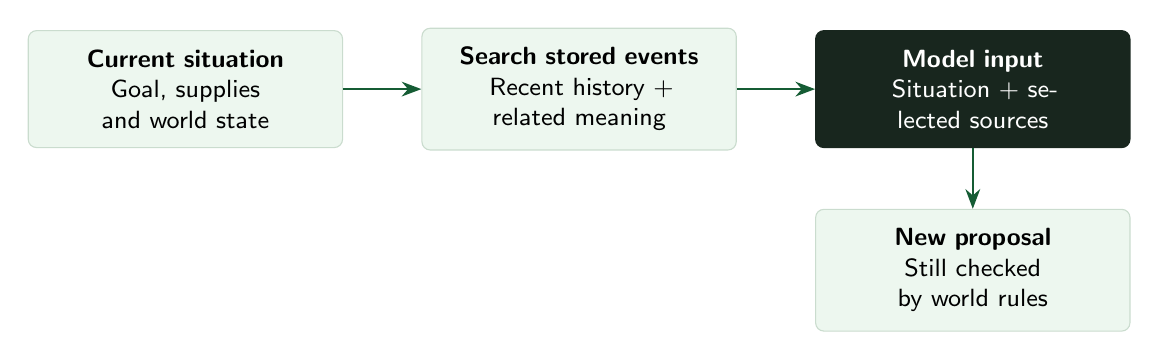
\begin{tikzpicture}
\node[card] (q) at (0,0) {\textbf{Current situation}\\Goal, supplies and world state};
\node[card] (s) at (5,0) {\textbf{Search stored events}\\Recent history + related meaning};
\node[darkcard] (c) at (10,0) {\textbf{Model input}\\Situation + selected sources};
\draw[arr] (q)--(s);\draw[arr] (s)--(c);
\node[card] (n) at (10,-2.3) {\textbf{New proposal}\\Still checked by world rules};
\draw[arr] (c)--(n);
\end{tikzpicture}}
\end{center}
\subhead{How meaning search helps}
"Collecting logs" and "gathering wood" can describe related ideas without using the same words. MiniLM converts text into number-based representations that help rank related events. We also keep recent history for immediate context.
\begin{saybox}
The full name is retrieval-augmented generation, or RAG. A simple analogy is taking an open notebook into a decision. First we find useful pages; then we give those pages to the model with the current situation.

Keyword search looks for matching words. Meaning search can find related wording, such as logs and wood. MiniLM helps with ranking, but our own code decides which events are eligible and how to assemble the context.

This differs from training. Looking up a memory changes the information given to the model for this decision. It does not rewrite the language model's weights.

Our retrieval checks found the expected source in all ten standard queries and all ten paraphrased queries. That shows lookup worked on those checks. It does not show that RAG always produces smarter or more cooperative behavior.
\end{saybox}
\begin{notebox}{Use this wording}
"A memory can inform the next decision." Avoid "The agent learned a new personality" or "This proves memory makes agents better."
\end{notebox}
\handoff{"Gayatri will explain a different ML job: sorting interactions."}

\pagehead{CLASSIFIER}{A sorter, not the decision-maker}{Gayatri}
\label{classifier}
\begin{center}
\resizebox{\linewidth}{!}{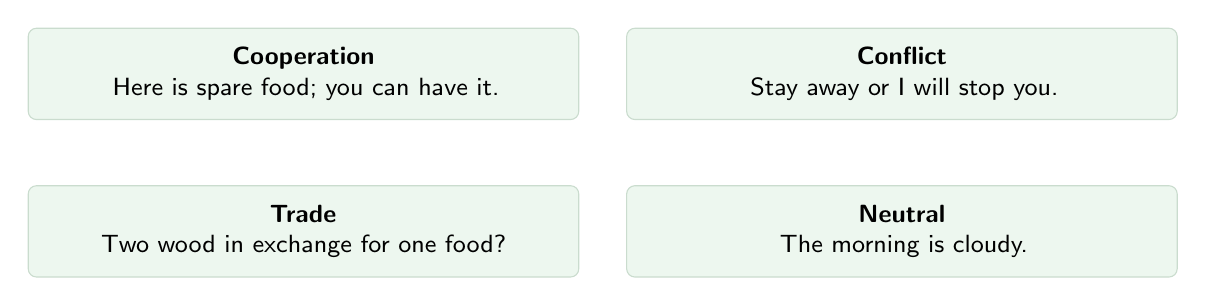
\begin{tikzpicture}
\node[card,text width=6.5cm] at (0,0) {\textbf{Cooperation}\\Here is spare food; you can have it.};
\node[card,text width=6.5cm] at (7.6,0) {\textbf{Conflict}\\Stay away or I will stop you.};
\node[card,text width=6.5cm] at (0,-2) {\textbf{Trade}\\Two wood in exchange for one food?};
\node[card,text width=6.5cm] at (7.6,-2) {\textbf{Neutral}\\The morning is cloudy.};
\end{tikzpicture}}
\end{center}
\captiontext{Illustrative sentences and intended categories. These are teaching examples, not a claim that the model predicts all four correctly.}
\begin{saybox}
The classifier has a narrower job than the language model. It reads an interaction and chooses a category: cooperation, conflict, trade or neutral.

Think of sorting messages into labelled trays. It does not write the town's next plan or decide how many coins anyone receives. It adds a label so we can inspect what kind of interaction happened.

We started with a small pre-trained model called DistilBERT. Pre-trained means it already has useful language patterns from earlier training. We adjusted it using our labelled town examples. That adjustment is fine-tuning.

The hosted Qwen model and this classifier are separate. We fine-tuned DistilBERT for sorting; we did not fine-tune Qwen for town decisions.
\end{saybox}
\subhead{Show the boundary}
\begin{center}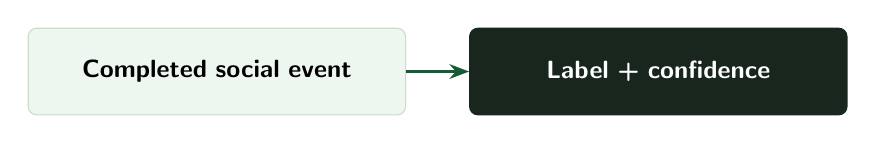
\begin{tikzpicture}
\node[card,text width=4.3cm] (a) {\textbf{Completed social event}};
\node[darkcard,text width=4.3cm,right=8mm of a] (b) {\textbf{Label + confidence}};
\draw[arr] (a)--(b);
\end{tikzpicture}\end{center}
\captiontext{The label follows execution. Inventory and relationships remain governed by world rules.}
\handoff{"Here is how we taught the sorter and checked its results."}

\pagehead{TRAINING}{Teach, choose, then test}{Gayatri}
\label{training}
\begin{center}
\resizebox{\linewidth}{!}{
\begin{tikzpicture}[x=.8cm,y=1cm]
\fill[forest] (0,0) rectangle (12,1.5);\fill[gold] (12,0) rectangle (16,1.5);\fill[ink] (16,0) rectangle (20,1.5);
\node[text=white,align=center,font=\bfseries] at (6,.75) {120 training\\examples};
\node[text=white,align=center,font=\bfseries] at (14,.75) {40 validation\\examples};
\node[text=white,align=center,font=\bfseries] at (18,.75) {40 test\\examples};
\node[align=center,text width=8cm,font=\small] at (6,-.7) {Teach the model};
\node[align=center,text width=3cm,font=\small] at (14,-.7) {Choose a saved version};
\node[align=center,text width=3cm,font=\small] at (18,-.7) {Check the frozen choice};
\end{tikzpicture}}
\end{center}
\subhead{Why three sets?}
If a student practices the exact exam questions, the exam tells us less about new material. Separate examples are used to fit the model, choose a checkpoint and evaluate the final frozen choice.

Related paraphrases stay together. Five rewrites of one situation should not be scattered across training and test.
\begin{saybox}
We have 200 short synthetic interactions, with 50 in each category. Synthetic means they were created for this project; this is not a large collection of real town conversations.

We used 120 examples for training and 40 validation examples to choose a saved model version, also called a checkpoint. Only after that choice did we evaluate the frozen model on 40 test examples.

We kept related versions of a situation in the same split. That reduces the chance that a test example is just a rewording of something used in training.

The available saved model had completed one training pass. We trained it for two additional passes for the presentation export. We started a new training setup from its saved internal settings, rather than claiming that we restored the entire earlier training process.
\end{saybox}
\begin{notebox}{Provenance note for questions}
The original checkpoint's dataset fingerprint was not supplied. The continuation used a fresh optimizer and the repository's exact frozen training split. Do not claim ten completed epochs from the original planned configuration.
\end{notebox}
\handoff{"Now we can compare the result with a simpler method."}

\pagehead{RESULTS}{What the classifier actually achieved}{Gayatri}
\label{results}
\begin{center}
\resizebox{\linewidth}{!}{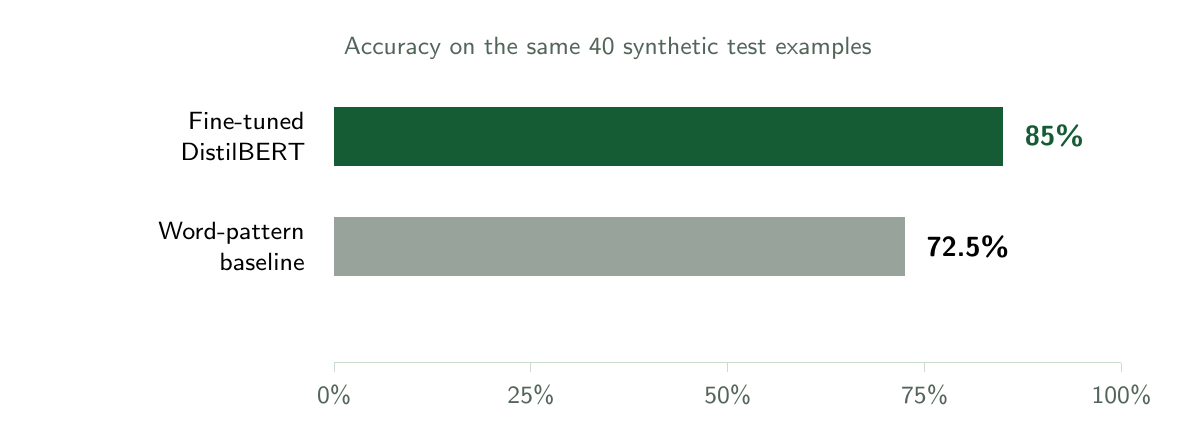
\begin{tikzpicture}[x=1cm,y=1cm]
\draw[line] (0,0)--(10,0);
\foreach \x/\lab in {0/0,2.5/25,5/50,7.5/75,10/100} {\draw[line] (\x,0)--(\x,-.12);\node[below,font=\small,text=muted] at (\x,-.15) {\lab\%};}
\fill[muted!60] (0,1.1) rectangle (7.25,1.85);\fill[forest] (0,2.5) rectangle (8.5,3.25);
\node[anchor=east,align=right,text width=3.4cm,font=\small] at (-.25,1.48) {Word-pattern\\baseline};
\node[anchor=east,align=right,text width=3.4cm,font=\small] at (-.25,2.88) {Fine-tuned\\DistilBERT};
\node[anchor=west,font=\bfseries] at (7.4,1.48) {72.5\%};
\node[anchor=west,font=\bfseries,text=forest] at (8.65,2.88) {85\%};
\node[anchor=west,font=\small,text=muted] at (0,4) {Accuracy on the same 40 synthetic test examples};
\end{tikzpicture}}
\end{center}
\begin{tabularx}{\linewidth}{@{}lYY@{}}
\toprule & \textbf{Simple baseline} & \textbf{DistilBERT}\\\midrule
Correct test examples & 29 of 40 & 34 of 40\\
Test macro-F1 & 0.709 & 0.850\\
\bottomrule
\end{tabularx}
\begin{saybox}
We compared the classifier with a simpler method based on word patterns and a basic statistical model. Both used the same data split.

The simpler baseline got 29 of the 40 test examples correct. DistilBERT got 34 correct, or 85 percent. Macro-F1 also balances different types of errors and gives each category equal weight.

These are useful results for this small project, not a claim of 85 percent accuracy on any conversation. Forty synthetic examples are a limited test.

We saw errors outside those examples too. A free-food gift was predicted as trade with low confidence, although its intended label was cooperation. A confidence number is the model's preference among labels, not a guarantee. That is why resource rules do not depend on the label.
\end{saybox}
\captiontext{Sources: classifier-test.json and classifier-validation.json in results/presentation/. Selection used validation before the test evaluation.}
\handoff{"Aishani and Saurya will show the system in action."}

\pagehead{LIVE DEMO}{Show one story, not every diagnostic}{Aishani / Saurya}
\label{demo}
\screen{demo-live.jpg}{7.5cm}
\captiontext{Actual simplified live view. Live plans, backup actions and the recorded example remain distinguishable.}
\begin{enumerate}
\item \textbf{Orient the room.} Choose Ethan and read the goal in ordinary language.
\item \textbf{Advance a turn.} Use Next Turn. Wait for an AI reply to be ready, then advance again if needed to execute it.
\item \textbf{Describe the result.} Follow the actual action; do not promise a conversation.
\item \textbf{Choose another resident.} Show its separate goal, supplies and story.
\item \textbf{Show the exchange.} Press Recorded example and select Ethan or Saurya.
\item \textbf{Name the switch honestly.} "This is a recorded, scripted example. It demonstrates the mechanics without new AI calls."
\end{enumerate}
\begin{saybox}
Here is the town running. We choose a resident and follow its goal and recent activity. When we advance a turn, the backend checks the action and the display updates.

The AI may choose to move, rest, gather or interact. We describe what appears rather than promising a specific outcome.

Now we switch to the labelled recorded example. This exchange is scripted so we can reliably show both sides of a trade and a conversation. It demonstrates the rules and interface, not an autonomous trade from this live run.
\end{saybox}
\handoff{"Aishani will explain what we would improve next."}

\pagehead{FURTHER DEVELOPMENT}{What we would improve next}{Aishani}
\label{future}
\begin{center}
\resizebox{\linewidth}{!}{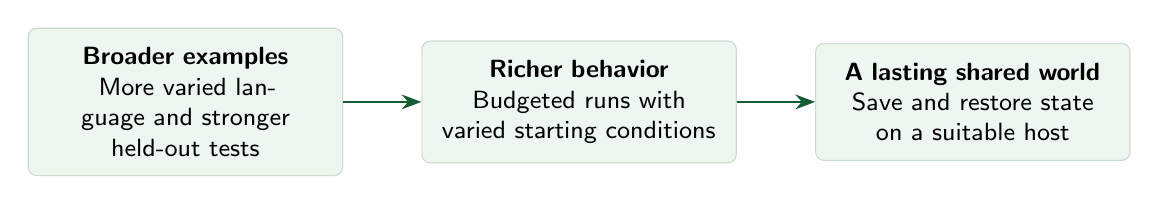
\begin{tikzpicture}
\node[card] (d) at (0,0) {\textbf{Broader examples}\\More varied language and stronger held-out tests};
\node[card] (b) at (5,0) {\textbf{Richer behavior}\\Budgeted runs with varied starting conditions};
\node[card] (w) at (10,0) {\textbf{A lasting shared world}\\Save and restore state on a suitable host};
\draw[arr] (d)--(b);\draw[arr] (b)--(w);
\end{tikzpicture}}
\end{center}
\subhead{Make each proposal measurable}
\begin{tabularx}{\linewidth}{@{}P{4cm}Y@{}}
\toprule\textbf{Proposed improvement} & \textbf{What counts as progress?}\\\midrule
More diverse labelled data & Better per-class results on genuinely new scenarios.\\
More reliable social behavior & Completed exchanges, legal proposals and fallback rates measured over controlled runs.\\
Better memory selection & Correct private sources, followed by measured decision quality.\\
Persistent hosting & World state survives restarts; viewers share a run without extra AI calls.\\
\bottomrule
\end{tabularx}
\begin{saybox}
Our next steps should improve things we can measure, rather than just make the town look busier.

First, we would expand the interaction dataset and test varied language. Mistakes show that examples outside our small dataset can still be difficult.

Second, we would run longer experiments with different starting resources and positions. We would measure completed trades, legal actions and how often the system falls back to rules. Our small comparison does not prove a benefit from memory.

Third, we would improve persistence and shared access. Restarting the backend currently starts a new town. A lasting shared world needs saved simulation state and reliable storage.

These are plans, not features we should claim are already completed.
\end{saybox}
\handoff{"Eric will connect those lessons to the original question."}

\pagehead{CLOSING}{Three ideas to leave with the audience}{Eric / host}
\label{closing}
\begin{center}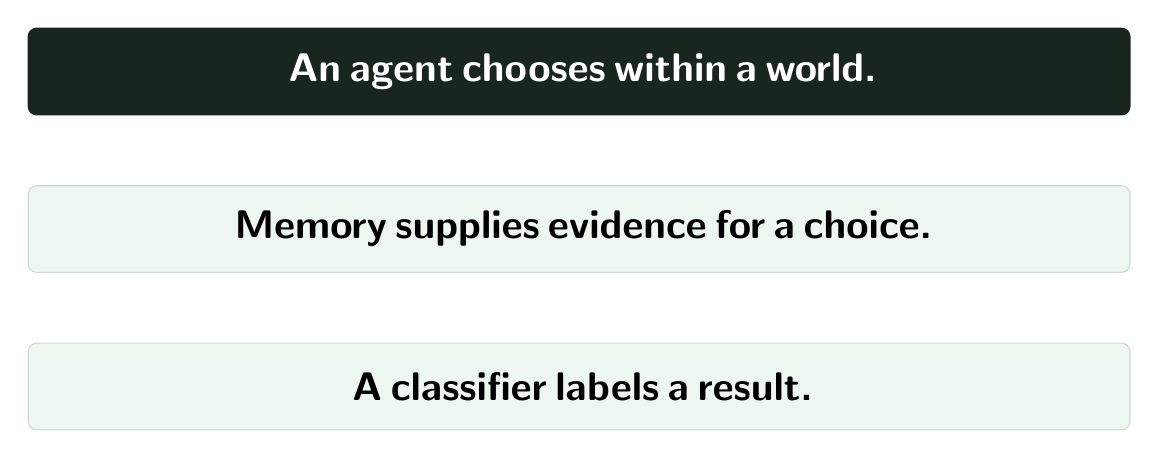
\begin{tikzpicture}
\node[darkcard,text width=13.5cm] at (0,0) {\Large\textbf{An agent chooses within a world.}};
\node[card,text width=13.5cm] at (0,-2) {\Large\textbf{Memory supplies evidence for a choice.}};
\node[card,text width=13.5cm] at (0,-4) {\Large\textbf{A classifier labels a result.}};
\end{tikzpicture}\end{center}
\begin{saybox}
MiniDavis helped us separate three ideas often grouped together as AI. An agent chooses an action. A memory system brings useful past evidence into that choice. A classifier gives an interaction a category.

The world engine connects those pieces by checking what is legal and recording what happens. That gives us something we can watch, test and explain.

Our strongest results are specific: working rules and retrieval checks, a small classifier evaluation and a visible interface. The next step is broader testing and more reliable long-running behavior.

Adding a model is only one part of an AI system. The surrounding rules, data, memory and evaluation determine whether its behavior is understandable and dependable.
\end{saybox}
\subhead{Closing slide idea}
One town image and these three statements. Keep the stack, scores and limitations in supporting material for questions.
\keyline{How can we make AI behavior visible enough to inspect, rather than simply trust?}

\pagehead{QUESTION BANK}{Answers for a non-ML audience}{Team reference}
\label{questions}
\subhead{"Are there five separate large AI models?"}
No. Five residents use one hosted Qwen service with separate contexts. They do not require five large models on a laptop.
\subhead{"Does the model see the town picture?"}
It receives text and numbers about the world. React draws the picture for humans; the model is not interpreting the screenshot.
\subhead{"What did you fine-tune?"}
DistilBERT, the small interaction classifier. The team did not fine-tune the hosted Qwen decision model.
\subhead{"Is saving a memory the same as training?"}
No. Saving changes a database. Retrieving changes the context for a later decision. Fine-tuning changes model weights.
\subhead{"How do you know a memory is real?"}
The engine writes events after execution. Retrieval checks the resident, run and event time. Presenter tools expose the source ID.
\subhead{"Why use a recorded example?"}
Live choices are unpredictable. A labelled scripted example reliably demonstrates mechanics, without claiming a live autonomous success.
\subhead{"Does 85 percent apply to any conversation?"}
No. It means 34 correct predictions on 40 synthetic test examples. More varied independent testing is needed.
\subhead{"Can a wrong label take someone's coins?"}
No. Inventory and relationships follow world rules. The classifier adds a label after an action.
\subhead{"What did the team build?"}
The simulation, interface, integration, storage/retrieval logic, data workflow and checks. Existing libraries, model architectures and pretrained weights are building blocks.

\pagehead{PRESENTER PREPARATION}{Set up off-stage; keep the screen simple}{Aishani / Saurya}
\label{preparation}
\begin{enumerate}
\item \textbf{Install and start the project.} Follow the root README. The trained model package is separate from Git.
\item \textbf{Check the backend.} Readiness should show the classifier loaded and semantic memory requested. A configured key alone does not prove a live response succeeded.
\item \textbf{Open Presenter tools.} Choose Live AI (Groq), start a new town and verify a real plan arrives. Use memory and classifier inspectors only for preparation.
\item \textbf{Close the tools.} The audience sees the map, resident stories and simple controls.
\item \textbf{Verify the example.} It should load with a recorded label and show the exchange. Reset or presenter setup returns to a fresh town.
\item \textbf{Agree on demo roles.} Aishani narrates and Saurya operates, or agree to swap before presenting.
\item \textbf{Check the real display and network.} Resident names, goals and stories must be readable from the audience's position.
\end{enumerate}
\subhead{If the service is unavailable}
Do not change secrets on stage or repeatedly press controls. Explain that the live service is unavailable or backup rules are in use. Switch to the labelled recorded example. Screenshots in this guide can also support the explanation.
\subhead{If an unexpected action appears}
Describe what actually happened. Continue the demonstration instead of forcing a particular model response.
\begin{notebox}{Keep private setup private}
The Groq API key stays on the backend. A protected shared town can use a different operator password. Neither credential belongs on a slide or in the public demo.
\end{notebox}
\subhead{Keep these out of the audience flow}
Model installation, API counters, classifier probe inputs, source IDs, memory query strings, revision numbers, seeds and long diagnostics. They stay under Presenter tools.

\pagehead{EVIDENCE AND LIMITS}{What the team can honestly claim}{Team reference}
\label{evidence}
\begin{tabularx}{\linewidth}{@{}P{4cm}Y@{}}
\toprule\textbf{Measured item} & \textbf{Observed result}\\\midrule
World/API/data tests & 152 passing checks in the recorded final audit.\\
Simplified frontend & 42 tests pass; production build passes.\\
Baseline stress run & 1,000 turns, no invariant failures, no provider calls.\\
Semantic retrieval & Expected source found in 10 standard and 10 paraphrased checks.\\
Classifier test & 34/40 correct; macro-F1 0.850. Baseline: 29/40, macro-F1 0.709.\\
Town comparison & 20/20 valid proposals across six exploratory runs. Three talks and two offers; no completed autonomous trade.\\
Local ML integration & Real CPU classification and semantic memory pass; a hosted service is not claimed.\\
\bottomrule
\end{tabularx}
\subhead{Limits that matter}
\begin{itemize}
\item The classifier test is small and synthetic. The source checkpoint's original dataset fingerprint was unavailable.
\item The town comparison has one planning window per live episode. Most later turns use cached plans or backup rules. It does not prove a causal RAG benefit.
\item The comparison's shortage operation found an already-empty farm. It does not measure a distinct shortage shock.
\item The recorded accepted exchange is scripted, not a completed autonomous trade from the comparison.
\item Automated checks do not establish public deployment, durable world restoration, venue rehearsal or a team-recorded video.
\end{itemize}
\begin{notebox}{A strong answer to "what did you learn?"}
"We learned to separate a model's proposal from a valid world action, a retrieved memory from training, and an attractive demo from measured evidence."
\end{notebox}

\pagehead{GLOSSARY AND SOURCES}{A shared vocabulary}{Team reference}
\label{glossary}
\begin{tabularx}{\linewidth}{@{}>{\bfseries}P{3.3cm}Y@{}}
Agent & A software resident that observes a situation and chooses an action.\\[3pt]
Model & A learned system mapping input to a prediction or response.\\[3pt]
LLM & A language model that can produce text, including a proposed action.\\[3pt]
Frontend & The interface people see and click.\\[3pt]
Backend & The service processing requests and owning world state.\\[3pt]
API & The agreed way to exchange requests and results.\\[3pt]
Memory & A stored event, filtered for the appropriate resident and run.\\[3pt]
Embedding & Numbers used to compare text by related meaning.\\[3pt]
RAG & Retrieve relevant information, then give it to a model as context.\\[3pt]
Fine-tuning & Adjust an existing model's weights with task-specific examples.\\[3pt]
Classifier & A model assigning an input to a category.\\[3pt]
Weights & The model's adjustable internal numbers, learned from examples.\\[3pt]
Cached plan & An earlier plan reused while it remains legal, such as travelling to a chosen location.\\[3pt]
Accuracy & The fraction of test examples classified correctly.\\[3pt]
Macro-F1 & A score balancing missed and incorrect predictions, giving each class equal weight.\\[3pt]
Fallback & Rules used when a live plan is unavailable or unusable.\\[3pt]
Replay & Saved actions executed without new AI decisions.\\
\end{tabularx}
\subhead{Evidence used in this guide}
\begin{itemize}
\item \href{https://github.com/KTH-Sys/MiniDavis}{MiniDavis repository}: current code and README.
\item \href{https://github.com/KTH-Sys/MiniDavis/blob/main/docs/model-card.md}{Model card}: provenance, continuation, test results and errors.
\item \href{https://github.com/KTH-Sys/MiniDavis/blob/main/results/presentation/classifier-test.json}{Classifier test report}: counts, per-class metrics and predictions.
\item \href{https://github.com/KTH-Sys/MiniDavis/blob/main/results/presentation/comparison/summary.json}{Comparison report}: calls, proposals, cached actions and fallback.
\item \href{https://github.com/KTH-Sys/MiniDavis/blob/main/results/presentation/retrieval.json}{Retrieval checks} and \href{https://github.com/KTH-Sys/MiniDavis/blob/main/docs/final-audit.md}{project audit}: sources and limitations.
\end{itemize}
\captiontext{Screenshots show the running app and label live versus recorded states. Diagrams explain the design; they are not additional experimental results. Artwork and font provenance are in the frontend asset documentation.}
\end{document}
